\chapter{Beschreibung einer Sicherheitsl\"ucke}
\label{chap:4}

Noch bevor eine endgültige Fassung des 5G-AKA Protokolls feststand haben sich einige Forscher bereits mit unterschiedlichen Sicherheitsaspekten des Protokolls auseinandergesetzt und teilweise sogar mögliche Sicherheitslücken entdeckt.
\textit{Martin Dehnel-Wild} und \textit{Cas Cremers} haben in \textit{Security vulnerability in 5G-AKA draft} solch eine Sicherheitslücke und dessen Auswirkungen, sowie mögliche Lösungsvorschläge vorgestellt. %Security vulnerability in 5G-AKA draft
Diese werden in diesem Kapitel vorgestellt.
Ihre Befunde beziehen sich auf die Spezifikation TS 33.501 V0.7.0 des 3GPP. %3GPP TS 33.501 V0.7.0
Mittlerweile hat das 3GPP bereits neuere Versionen der Spezifikation veröffentlicht, darunter auch die Version V15.34.1, auf der die Beschreibung aus \cref{chap:2} beruht. %3GPP TS 33.501 V15.34.1
Zur Verbesserung der Übersichtlichkeit wird daher im weiteren Verlauf die Sicherheitslücke im Kontext der Spezifikation TS 33.501 V15.34.1 beschrieben.


\section{Beschreibung der Sicherheitslücke}

\begin{figure}[H]
  \centering
  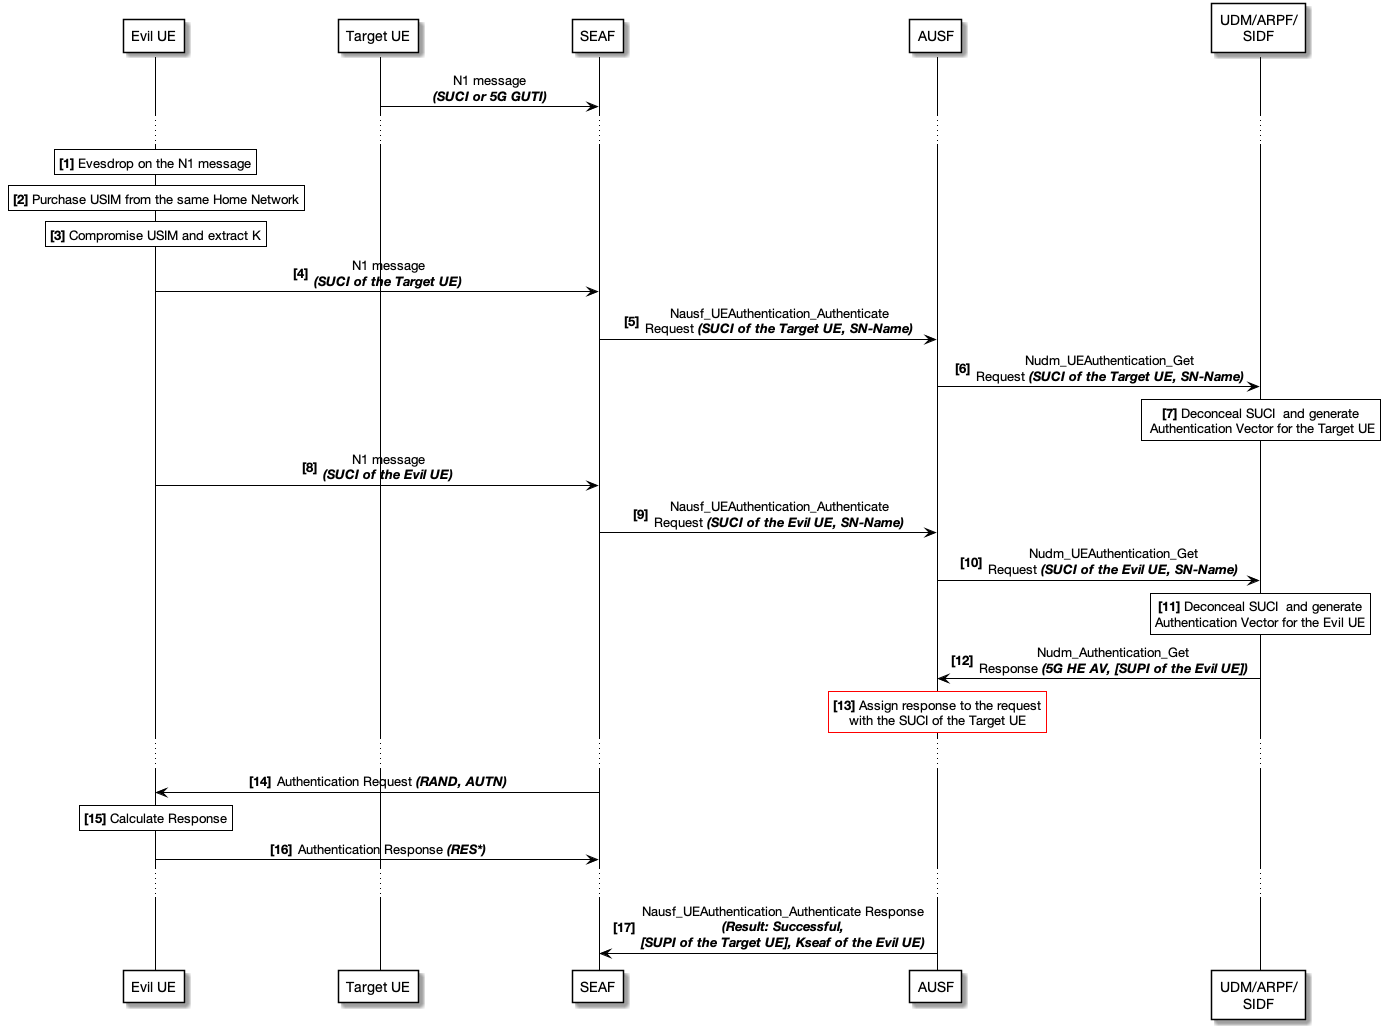
\includegraphics[width=\textwidth]{uml/vulnerability_v1.png}
  \caption{Beschreibung der Sicherheitslücke}
  \label{fig:vulnerability_v1}
\end{figure}

Die in dem \textit{Security vulnerability in 5G-AKA draft} vorgestellte Sicherheitslücke ermöglicht es einem Angreifer sich als ein anderer Benutzer auszugeben. %Security vulnerability in 5G-AKA draft
Zur Vereinfachung wird hier davon ausgegangen, dass das \gls{udm}/\gls{arpf}/\gls{sidf} immer das 5G-AKA Protokoll auswählt und nicht das EAP-AKA' Protokoll.
Hierbei handelt es sich um eine \textit{Race Condition}.
Der Angriff funktioniert also nicht in allen Versuchen.
Bevor er jedoch ausgeführt werden kann müssen einige Vorbereitungen getroffen werden.

\subsection{Vorbereitungen}

\begin{enumerate}
%1
\item Der Angreifer muss an den \gls{suci} des Benutzers kommen für den er sich ausgeben möchte.
Dafür muss er die \textit{N1 message} des Benutzers mithören und aufzeichnen.

%2
\item Hat der Angreifer die \textit{N1 message} des Benutzers aufgezeichnet, dann bringt er in Erfahrung zu welchem \textit{Home Network} der \gls{suci} gehört und kauft sich ein legitimes \gls{usim} des selben \textit{Home Network}s.

%3
\item Ist der Angreifer im Besitz des legitimen \gls{usim} so kompromittiert er dieses und extrahiert daraus den Langzeitschlüssel \gls{k}.

\end{enumerate}

\subsection{Der Hauptteil des Angriffs}

\begin{enumerate}
\setcounter{enumi}{3}

%4
\item Der Angreifer sendet nun eine \textit{N1 message} an die \gls{seaf} und initiiert somit eine neue Authentifikation.
Diese Nachricht enthält den \gls{suci} des Benutzers, den der Angreifer in \textit{Schritt 1} abgehört hat.

%5
\item Der \gls{suci} des abgehörten Benutzers wird von der \gls{seaf} an die \gls{ausf} weitergeleitet.

%6
\item Das \gls{udm} erhält den \gls{suci} des abgehörten Benutzers und beginnt die erhaltene Nachricht zu verarbeiten.

%7
\item Das \gls{udm} berechnet den \gls{supi} des abgehörten Benutzers aus dem \gls{suci} den es in \textit{Schritt 6} erhalten hat und generiert einen Authentifikations-Vektor für den \gls{suci} des abgehörten Benutzers.

%8
\item Direkt nach dem versenden der Nachricht aus \textit{Schritt 4} sendet der Angreifer erneut eine \textit{N1 message} jedoch dieses mal mit dem \gls{suci} des \gls{usim}s das er in \textit{Schritt 2} gekauft hat.

%9
\item Auch der \gls{suci} des Angreifers wird von der \gls{seaf} an die \gls{ausf} weitergeleitet.

%10
\item Das \gls{udm} erhält den \gls{suci} des Angreifers kurz nachdem es den \gls{suci} des abgehörten Benutzers erhalten hat.

%11
\item Das \gls{udm} berechnet den \gls{supi} des Angreifers aus dem \gls{suci}, den es in \textit{Schritt 9} erhalten hat und generiert den Authentifikations-Vektor  für den \gls{suci} des Angreifers.

%12
\item Das \gls{udm} hat in \textit{Schritt 7 \& 11} erst den \gls{suci} des abgehörten Benutzers und dann den \gls{suci} des Angreifers erhalten.
Nun sendet es aber erst den Authentifikations-Vektor für den \gls{suci} des Angreifers an die \gls{ausf} zurück.
Das \gls{udm} sendet also die Antworten auf die erhaltenen Nachrichten nicht in der gleichen Reihenfolge zurück in der es die \gls{suci}s erhalten hat.

In diesem Schritt (Schritt 12) wird in der hier beschriebenen Version(V15.34.1) zusätzlich zu dem \gls{5g-he-av} auch unter bestimmten Umständen der \gls{supi} mitgesendet.
Dies ist bei der Version(V0.7.0), auf der in dem \textit{Security vulnerability in 5G-AKA draft} eingegangen wird, nicht der Fall.

%13
\item Die \gls{ausf} erhält nun zuerst die Antwort auf die Nachricht aus \textit{Schritt 11}.
Da die Antwort des \gls{udm} nicht den \gls{suci} enthält kann die \gls{ausf} nicht überprüfen zu welchem \gls{suci} die Antwort gehört und nimmt daher fälschlicherweise an, dass die erhaltene Antwort zur Nachricht aus \textit{Schritt 6} gehört.

%14
\item In Schritt 14 erhält der Angreifer von der \gls{seaf} den Authentication Request.
Diese Nachricht enthält nun \gls{rand} und \gls{autn} die das \gls{udm} für den \gls{suci} des Angreifers, die \gls{seaf} jedoch nimmt an, das \gls{rand} und \gls{autn} für die Authentifizierung des abgehörten Benutzers bestimmt sind.

%15
\item Der Angreifer kann nun \gls{res*} aus \gls{rand} und \gls{autn} berechnen, da er in \textit{Schritt 3} den dafür benötigten Langzeitschlüssel \gls{k} erhalten hat.

%16
\item Der Angreifer sendet nun die in \textit{Schritt 15} berechnete \gls{res*} an die \gls{seaf}.

%17
\item Die \gls{seaf} und die \gls{ausf} überprüfen nun die \gls{res*} aus \textit{Schritt 16} und akzeptieren sie schließlich.
Das 5G-AKA Protokoll wurde also erfolgreich ausgeführt.
Jedoch nehmen \gls{seaf} und \gls{ausf} an, dass sich der abgehörte Benutzer erfolgreich authentifiziert hat und nicht der Angreifer.
Der Angreifer kann sich nun also dem \gls{seaf} gegenüber als den abgehörten Benutzer ausgeben.

Auch in diesem Schritt (Schritt 16) wird in der hier beschriebenen Version(V15.34.1) unter bestimmten Umständen der \gls{supi} mitgesendet nachdem er in \textit{Schritt 12} zwischengespeichert wurde.
Dies ist bei der Version(V0.7.0), auf der in dem \textit{Security vulnerability in 5G-AKA draft} eingegangen wird, nicht der Fall.


\end{enumerate}


\section{Verletzte Eigenschaft}

Nachdem der Angriff erfolgreich ausgeführt wurde sich die \gls{seaf}, die \gls{ausf} und der Angreifer im Besitz des \textit{''Anchor Key''}s \gls{k-seaf} und haben sich auf diesen geeinigt.
Des Weiteren sind glauben \gls{seaf} und die \gls{ausf}, dass der \gls{k-seaf} nur im Besitz des angehörten Benutzers und nicht im Besitz des Angreifers ist.

Es wird also die Eigenschaft verletzt, dass der \textit{''Anchor Key''} \gls{k-seaf} geheim seien soll.

Ein Angreifer kann somit, sofern er im Besitz eines beliebigen validen Langzeitschlüssels \gls{k} ist, sich als jeden anderen Benutzer ausgeben, der bei dem gleichen Provider eine \gls{usim} gekauft hat und dessen \gls{suci} dem Angreifer bekannt ist.


\section{Auswirkungen der Sicherheitslücke}

Diese Sicherheitslücke erlaubt es einem Angreifer sich als einen anderen Benutzer auszugeben.
Der Angriff kann unabhängig von der beim \gls{suci} verwendeten \textit{Protection Scheme} erfolgreich ausgeführt werden, es ist also nicht notwendig dass für die Verschlüsselung des \gls{suci} der \textit{Null Scheme} verwendet wurde.
Da der Angriff auf einer \textit{Race Condition} beruht kann nicht garantiert werden, dass er bei jedem Durchlauf erfolgreich durchgeführt wird.

Dieser Angriff erlaubt es nicht die Nachrichten zwischen einem abgehörten Benutzer und der \gls{seaf} zu entschlüsseln.

Ein Angreifer könnte sich jedoch als einen anderen Benutzer ausgeben und auf seinen Kosten Dienstleistungen des Providers in Anspruch nehmen.

Durch die Implementierung und andere technische Maßnahmen kann eine erfolgreiche Durchführung des Angriffs verhindert werden und somit verhindert werden das sich ein Angreifer als einen anderen Benutzer ausgibt.

In der hier beschriebenen Version(V15.34.1) wird in \textit{Schritt 7 \& 17} aus \cref{fig:protocol_v1} unter bestimmten Umständen auch der \gls{supi} mitgesendet.
Dies ist in der im \textit{Security vulnerability in 5G-AKA draft} betrachteten Version(V0.7.0) nicht der Fall und könnte die Funktionalität der Sicherheitslücke beeinträchtigen.


\section{Beschriebene Lösungsvorschläge}

\textit{Martin Dehnel-Wild} und \textit{Cas Cremers} haben in dem \textit{Security vulnerability in 5G-AKA draft} verschiedene Lösungsvorschläge beschrieben.

In dem ersten Lösungsansatz wird vorgeschlagen, dass in der \textit{Nudm\_Authentication\_Get Response} Nachricht aus \textit{Schritt 7} in \cref{fig:protocol_v1} zusätzlich \gls{suci} \& \gls{supi} und dass in der \textit{Nausf\_UEAuthentication\_Authenticate Response} Nachricht aus \textit{Schritt 10} aus \cref{fig:protocol_v1} zusätzlich der \gls{suci} mitgesendet wird.
Dies ermöglicht es der \gls{ausf} und der \gls{seaf} die erhaltenen Nachrichten eindeutig zuzuordnen und somit einen erfolgreichen Angriff zu verhindern.

Ein anderer Lösungsansatz schlägt vor, dass die Nachrichten zwischen der \gls{ausf} und der \gls{arpf} eine eindeutige Zufallszahl enthalten und somit klar zugeordnet werden können.






